\section{Background and Scope}

BaZn$_2$Si$_2$O$_7$ is a silicate in the BaO--ZnO--SiO$_2$ system that undergoes a reversible structural transition. Its low-temperature phase shows pronounced positive thermal expansion, whereas the high-temperature phase that forms on heating can show near-zero or negative thermal expansion, which makes the compound a model system for studying tetrahedral-chain flexibility and compositional tuning. Lin et al. resolved the transition and both crystal structures by high-temperature X-ray diffraction (HT\nobreakdash-XRD), providing the structural benchmark for the phase-control studies that followed \cite{lin1999phase}.

This review is organized around three questions: how the structure and synthesis conditions of BaZn$_2$Si$_2$O$_7$ jointly determine the main phase; how far Ba\slash Sr, Zn\slash Mg\slash Co\slash Ni\slash Cu, and Si\slash Ge substitution can tune phase stability; and what verifiable grounds exist for treating Ba$_5$Y$_{12}$Zn[O(SiO$_4$)]$_8$ as a structural analogue. Public databases confirm that BaZn$_2$Si$_2$O$_7$ is orthorhombic, that Ba is five-coordinate, and that the ZnO$_4$ and SiO$_4$ tetrahedra form a corner-sharing network \cite{available2020materials}, but our search turned up no verifiable primary crystallographic paper on Ba$_5$Y$_{12}$Zn[O(SiO$_4$)]$_8$. Throughout, we therefore keep ``direct reports'', ``structurally related compounds'', and ``structural inference'' strictly apart.

The structurally related compounds are more than background. Work on Ba$_{1-x}$Sr$_x$Zn$_2$Si$_2$O$_7$ shows that a small amount of Sr is enough to stabilize the high-temperature structure down to room temperature and to push the thermal expansion coefficient into the negative range \cite{thieme2015ba1,thieme2016very}, and aliovalent or isovalent substitution on the Zn site further shifts the transition temperature and the anisotropy \cite{thieme2016new,kerstan2013bazn2si2o7}. These findings supply transferable structure--processing correlations against which the target analogue can be compared; they do not imply that Ba$_5$Y$_{12}$Zn[O(SiO$_4$)]$_8$ has been synthesized.

Figure~\ref{fig:roadmap} lays out the order in which these topics are treated, and Figure~\ref{fig:taxonomy} places structure, synthesis, phase control, and evidence boundaries in a single framework.

\begin{figure}[t]
  \centering
  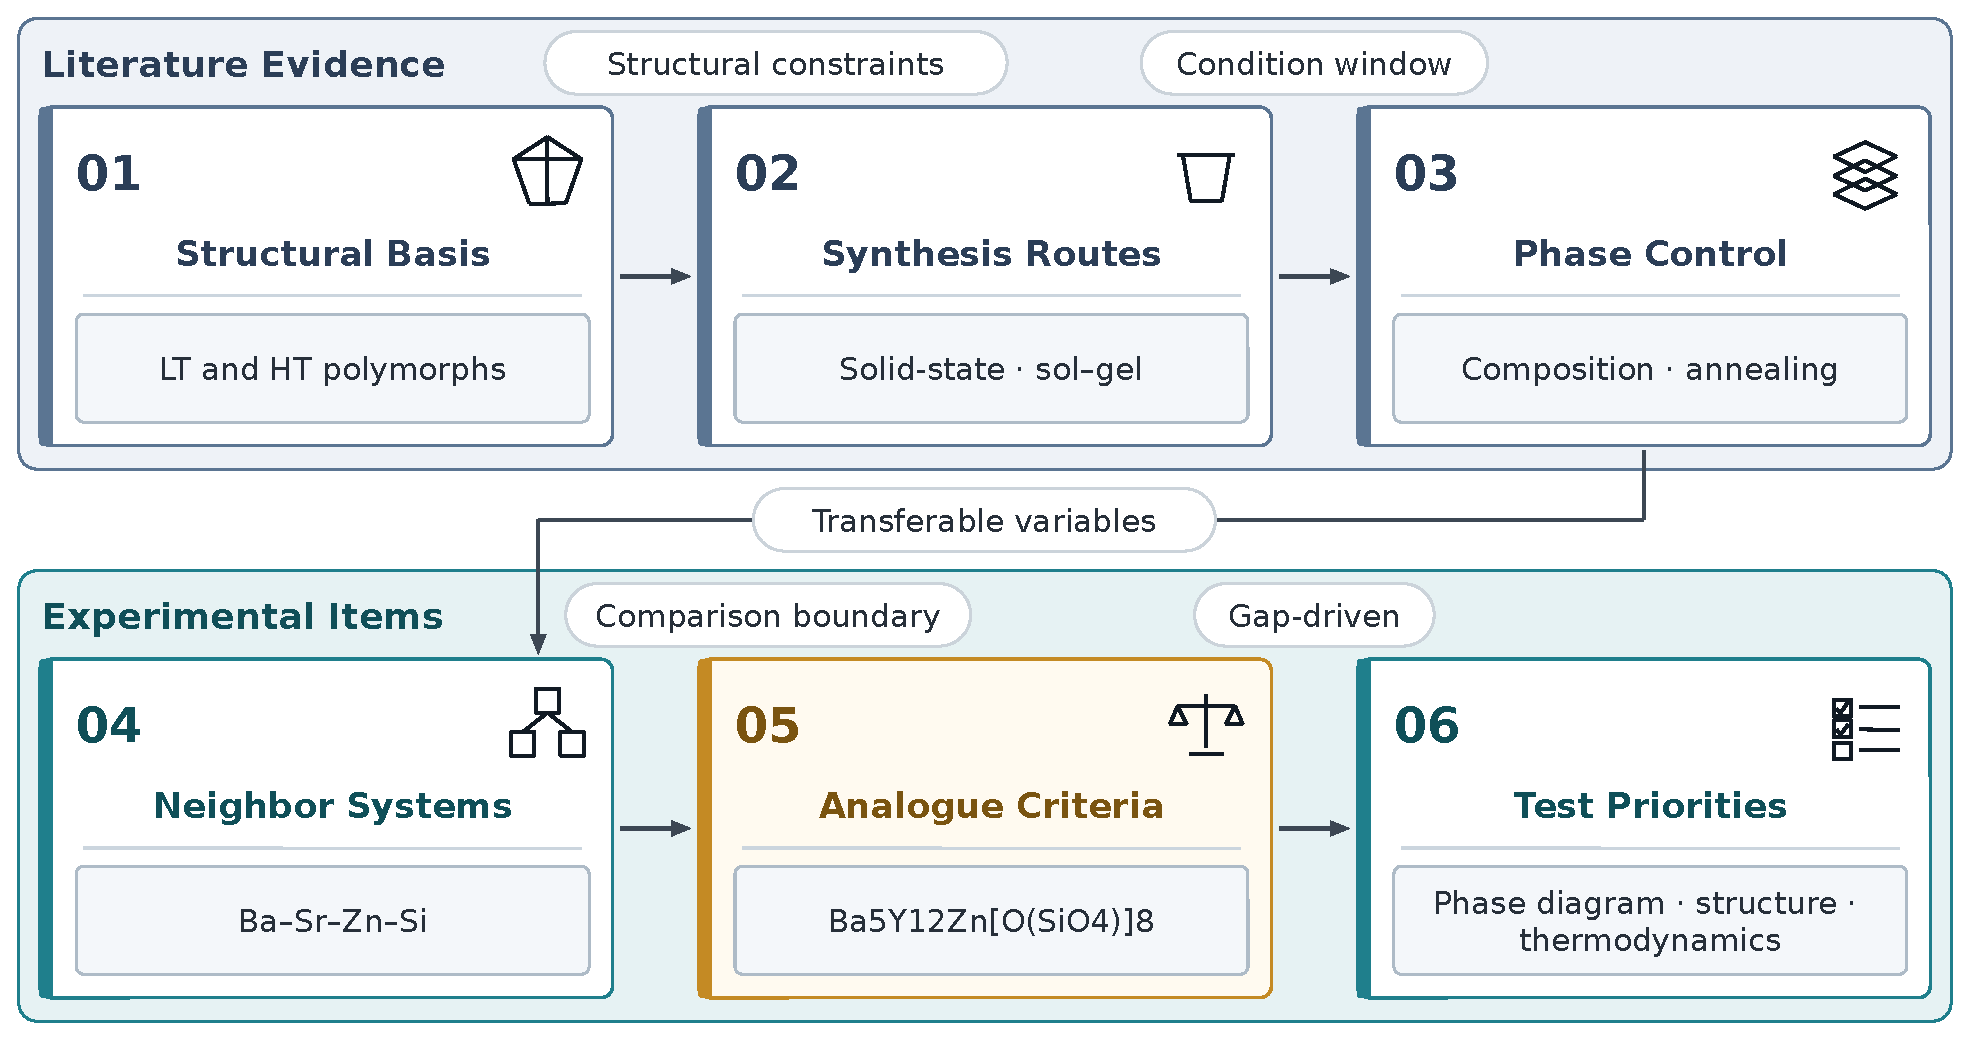
\includegraphics[width=\linewidth]{../figures/pdf/roadmap_bazn2si2o7_en.pdf}
  \caption{\textbf{Roadmap of this review.} Arrows trace the progression from structural facts to synthesis windows, to trends transferred from structurally related compounds, and finally to falsifiable experimental recommendations.}
  \label{fig:roadmap}
\end{figure}
